\chapter{การเรียนรู้แบบลึก}
\label{chapter: ANN deep learning}
\index{deep learning}

\begin{verse}
``What you get by achieving your goals is not as important as what you become by achieving your goals.'' \\
Johann Wolfgang von Goethe
\end{verse}

โครงข่ายประสาทเทียม ความลึก $2$ ชั้น นั้น แม้จะสามารถทำงานหลายๆอย่างได้ดี ดังที่เห็นไปเช่น ตัวอย่างในบท~\ref{chapter: Applications of ANN}.
แต่ ความสามารถของ โครงข่ายประสาทเทียม ก็ยังห่างไกลจากเป้าหมายสูงสุด ของ ศาสตร์ปัญญาประดิษฐ์ ซึ่งคือ การสร้างเครื่องจักรที่มีความฉลาด เทียบเท่า ความฉลาดของมนุษย์.
มีความพยายามศึกษาหลายๆ แนวทาง เพื่อไปสู่เป้าหมายนั้น เช่น แนวทาง (Artificial General Intelligence)\cite{AGI2007a} , แนวทางที่พยายามจะรวม connectionism และ symbolism เข้าด้วยกัน\cite{Smolensky1988a, Smolensky1990a, ParkEtAl1995a}, แนวทางที่พยายามสร้างกรอบทำงานเชิงคำนวณรวมทั่วไป (generic computational framework)\cite{Prokopenko2014a}, แนวทางของ reinforcement learning, แนวทางของ hierarchical learning \cite{TaniNolfi1999a}, แนวทางการใช้บริบทประกอบ (context-aware learning)\cite{Turney1993a, SongEtAl2002a, FinkelEtAl2004a, SrinivasanEtAl2005a, GomesEtAl2011a} และ การเชื่องโยง มโนทัศน์ที่คล้ายคลึงกัน ในมุมมองต่างๆ, เป็นต้น รวมไปถึง การพยายาม จะนำ มิติที่เชื่อว่าจะช่วยเสริม ความสามารถ ของโครงข่ายประสาทเทียมไปในแนวทางนั้น เช่น active learning, transfer learning, เป็นต้น

ถึงแม้จะมีความพยายามดังกล่าวมานี้ สถานะปัจจุบัน ของศาสตร์และศิลป์ ของวิทยาการปัญญาประดิษฐ์ ก็ยังห่างไกล จากเป้าหมายสูงดังกล่าว.

\begin{verse}
``Only a small community has concentrated on general intelligence.
No one has tried to make a thinking machine . . .
The bottom line is that we really haven't progressed too far toward a truly intelligent machine. 
We have collections of dumb specialists in small domains; 
the true majesty of general intelligence still awaits our
attack. . . .
We have got to get back to the deepest questions of AI and general
intelligence...''
\\– Marvin Minsky
\\as interviewed in Hal’s Legacy, edited by David Stork, 2000.
\end{verse}

อย่างไรก็ดี ความก้าวหน้าล่าสุด ที่สร้างความตื่นเต้น กับ วงการปัญญาประดิษฐ์ และ คอมพิวเตอร์โดยรวม ไปจนถึง ผู้สนใจทั่วไป คือ แนวทางของการเรียนรู้เชิงลึก (Deep Learning) ที่นอกจากจะทำงานในลักษณะการเรียนรู้แบบมีผู้สอนได้ดีแล้ว ยังเสมือนเป็นการรวมการการเรียนรู้แบบไม่มีผู้สอนเข้าไปได้ด้วย และ ยังเปิดทางให้กับ การทำ transfer learning, และ hierarchical representation ด้วย.
หากจะเริ่มต้น กล่าวถึง การเรียนรู้เชิงลึก, แม้แนวคิดจะมีมานานมากพอๆกับ จุดกำเนิดของโครงข่ายประสาทเทียมเอง และ วิธีการแพร่กระจายย้อนกลับเองก็สามารถนำมาใช้ได้.
แต่การประยุกต์ใช้ โครงข่ายประสาทเทียมแบบลึก นั้นจำกัดอยู่มาก, จนกระทั่งการค้นพบที่สำคัญ ในปีี 2006 \cite{HintonSalakhutdinov2006a} ที่พบ วิธีการฝึกโครงข่ายประสาทเทียมแบบลึกได้อย่างมีประสิทธิภาพ.
หลักจากนั้น ก็มีการศึกษา การเรียนรู้แบบลึก อย่างกว้างขว้าง และ การเรียนรู้แบบลึก ก็กลายเป็น ศาสตร์และศิลป์ ที่สำคัญ สำหรับ ศาสตร์หลายๆแขนง \cite{Jones2014a, Schmidhuber2015a,MNIST20150311,DahlSainathHinton2013a,DengEtAl2013a, 
ErhanEtAl2010a,CaetanoDosSantoEtAl2015,RamsundarEtAl2015,
ChenEtAl2014a,MaEtAl2015a,XiongEtAl2015a} เช่น computer vision, speech recognition, natural language processing, drug discovery เป็นต้น.
การเรียนรู้แบบลึก มีความสำคัญ มีการใช้งานที่กว้างขวาง และศักยภาพสูงมาก จน
MIT Technology Review 2013 ได้ยกให้ การเรียนรู้แบบลึก (deep learning) เป็น 1 ใน 10 breakthroughs ของปี 2013.
ในขณะที่ รายการของปี 2014 ได้ยกให้ Neuromorphic Processing Unit เป็น 1 ใน breakthorughs ของปี.
Neuromorphic Processing Unit (NPU) \cite{MerollaEtAl2014a} ซึ่งคือ ฮาร์ดแวร์ที่โครงสร้างออกแบบเฉพาะ สำหรับ การใช้งานโครงข่ายประสาทเทียมหลากหลายรูปแบบ (รวมถึง โครงสร้างแบบลึก).
สถาปัตยกรรมนี้ ต่างจาก von Neumann machine ที่เป็นแนวคิดหลักของคอมพิวเตอร์ในปัจจุบัน อย่างสิ้นเชิง.
ผู้อ่านที่สนใจ เรื่อง NPU สามารถศึกษาได้ จาก งานที่สำคัญของ เมอโรลาและคณะ จาก IBM \cite{MerollaEtAl2014a}.

หัวข้อ~\ref{deep learning: self-taught learning} อภิปรายแนวคิดของ self-taught learning ซึ่งเป็นงานศึกษาถึงการใช้ การเรียนรู้แบบไม่มีผู้สอน มาช่วยเรียนลักษณะที่สำคัญของข้อมูล เพื่อ เพิ่มประสิทธิภาพในการเรียนรู้แบบมีผู้สอน.
เนื้อหา self-taught learning นำมาจาก บทความของรายนะและคณะ\cite{RainaEtAl2007a}.
โดยถึงแม้ งานของรายนะและคณะ จะเป็นโมเดลเชิงเส้น ที่มีลักษณะตื้น แต่ หลักการที่ นำข้อมูลไม่มีฉลาก มาปรับโมเดล ยกหนึ่งก่อน เพื่อที่จะหา representations ที่ดีของข้อมูล,
ซึ่งภายหลัง representations ที่ดี จะช่วยให้ การปรับโมเดลอย่างละเอียด ด้วย ข้อมูลที่มีฉลาก จะทำได้มีประสิทธิภาพ มากขึ้น.
แนวคิดนี้ เป็นหลักการเดียวกันกับ แนวทาง ที่นำมาใช้กับการฝึกโครงสร้างแบบลึก ด้วยการทำ pre-train ที่จะกล่าวต่อไปในหัวข้อ~\ref{deep learning: autoencoder}.

\section{การเรียนรู้แบบสอนตนเอง}
\label{deep learning: self-taught learning}
\index{self-taught learning}

เนื้อหาในหัวข้อนี้ มาจากงานของ รายนะและคณะ \cite{RainaEtAl2007a} ที่ศึกษา การนำ ข้อมูลที่ไม่มีฉลาก มาช่วยเพิ่มประสิทธิภาพ การเรียนรู้แบบมีผู้สอน. 
%ที่ต้องการข้อมูลพร้อมฉลาก 
และ เสนอแนวทาง ที่เรียกว่า ``self-taught learning'' หรือ ``การเรียนรู้แบบสอนตนเอง''.

\paragraph{Conventional supervised learning:} สถานการณ์ที่ทำๆกันมา ของ การทำโมเดล สำหรับ งานการเรียนรู้แบบมีผู้สอน คือ เราจะมี ข้อมูลตัวอย่าง พร้อมกับ เฉลย ที่มักเรียก ``ฉลาก'':
งานหาค่าถดถอย, ฉลาก ก็คือ ค่าเอาต์พุต ที่ต้องการ;
งานจำแนกกลุ่ม, ฉลาก ก็คือ กลุ่มที่ถูกต้อง.

\paragraph{Issue:} ดังนั้น หากจะทำ การทำโมเดล สำหรับ งานการเรียนรู้แบบมีผู้สอน, เราต้องมี ตัวอย่างที่ดี และ เพียงพอ: มี ข้อมูลตัวอย่าง พร้อม ฉลาก และ ตัวอย่างก็ควรจะมีจำนวน และ ความหลากหลายเพียงพอ ที่จะช่วยให้ โมเดลได้เรียนรู้ ความน่าจะเป็น ของ ความสัมพันธ์ ระหว่างข้อมูลและฉลาก, การกระจายของข้อมูล, และ การกระจายของฉลาก.
แต่ สำหรับ งานหลายๆประเภท เช่น การรู้จำวัตถุ (object recognition), การรู้จำเสียง (speech recognition), การจำแนกชนิดบทความ (text article classification), การแปลภาษา (machine translation), เป็นต้น, สถานการณ์ คือ มันเป็นงานที่ซับซ้อน และต้องการข้อมูลตัวอย่างจำนวนมาก;
แต่ ข้อมูลที่มีฉลาก (ที่ถูกต้อง และ เกี่ยวข้อง) มีจำนวนน้อย เกินไป ที่จะใช้ทำโมเดลที่ดีได้.
อย่างไรก็ตาม โอกาสก็คือ มี ข้อมูลที่ไม่มีฉลาก เป็นจำนวนมาก (มี รูปภาพ, ไฟล์เสียง, บทความ ข้อเขียน ข้อความ ต่างๆ อยู่มากมาย หลากหลายภาษา ในอินเตอร์เนต).
งานการเรียนรู้แบบมีผู้สอน แบบดั้งเดิม ไม่ได้ใช้ประโยชน์ จาก ข้อมูลที่ไม่มีฉลากที่มีอยู่เป็นจำนวนมาก เหล่านี้ เลย.

\paragraph{Proposed solution:} แนวคิด ของ self-taught learning คือ การใช้ ข้อมูลที่ไม่มีฉลาก เช่น รูปภาพ (หรือ ไฟล์เสียง หรือ เอกสารข้อความ) มาช่วยในการปรับโมเดลก่อน.
นำข้อมูลไม่มีฉลากจำนวนมาก จะปรับให้โมเดลสรุปได้ลักษณะที่สำคัญ ของข้อมูลมาก่อน
แล้วค่อย นำข้อมูลที่มีฉลาก มาปรับแต่งโมเดลในขั้นตอนสุดท้าย เพื่อให้ได้งานที่ต้องการ.

โดย รายนะและคณะ ได้แจกแจงความแตกต่างระหว่าง self-taught learning กับ งานการเรียนรู้ของเครื่องแบบอื่นๆ เช่น supervised learning (งานเรียนรู้แบบมีผู้สอน), semi-supervised learning (งานเรียนรู้แบบกึ่งมีผู้สอน), transfer learning (งานโยกย้ายการเรียนรู้) พร้อมภาพประกอบ ที่แสดงในรูป~\ref{fig: deep self-taught compares}.
หากต้องการสร้างโมเดล เพื่อ แยกภาพของ ช้าง กับ แรด,
supervised learning ต้องการ ภาพตัวอย่าง ของทั้งช้าง และ แรด พร้อม ฉลาก ระบุว่า เป็นภาพ ช้าง หรือ แรด จำนวนมาก;
semi-supervised learning\footnote{
เช่น เราใช้ ภาพของช้างกับแรดที่มีฉลาก มาฝึกโมเดล และ ทายฉลาก ของภาพที่ไม่มีฉลาก;
แล้ว ใช้ ภาพที่ไม่มีฉลาก มาประกอบกับ ฉลากที่ทาย มาฝึกโมเดลต่อ.
ทำเช่นนี้ จะเสมือนว่า เราได้มีข้อมูลที่มีฉลากเยอะขึ้น.
ดู [cite Tom Mitchell's semisupervised learning] เพิ่มเติมสำหรับ Semi-supervised learning.} 
ต้องการ ภาพตัวอย่าง ของทั้งช้าง และ แรด ที่มี ฉลาก และ สามารถเสริมด้วย ภาพช้าง และ ภาพแรด ที่ไม่มีฉลากได้;
transfer learning\footnote{
ดู [cite Quan Yan's Transfer Learning] เพิ่มเติมสำหรับ Transfer learning.
}
ต้องการ ข้อมูลตัวอย่างของงานที่ต้องการ พร้อมฉลาก และ สามารถเสริมได้ด้วย ตัวอย่างของงานที่คล้ายคลึงกัน
เช่น สมมติว่า งานจำแนกม้าและแพะ สามารถนำมาช่วย งานจำแนกช้างและแรดได้,
transfer learning ก็สามารถใช้ ภาพแพะ และ ภาพม้า พร้อมฉลาก มาเสริมได้;
รายนะ และ คณะ ชี้แจงว่า self-taught learning เหมาะสมกับ สภาพทั่วๆไปมากกว่า คือ สำหรับ งานจำแนกช้างและแรด, seft-taught learning สามารถใช้ ภาพอะไรก็ได้มาเสริมการทำงาน โดย 
ไม่จำเป็นว่า ภาพที่มาเสริมจะต้องเป็น ภาพช้าง หรือ ภาพแรด (เงื่อนไขของ semi-supervised learning)
หรือ
ไม่จำเป็นว่า ภาพที่มาเสริมจะต้องมีฉลากประกอบ (เงื่อนไขของ transfer learning).

%
\begin{figure}
\begin{center}
\includegraphics[width=5.5in]{04ANNDeep/MLCompare.png}
\end{center}
\caption{ภาพจาก Raina et al 2007 เปรียบเทียบ supervised learning, semi-supervised learning, transfer learning, และ self-taught learning.}
\label{fig: deep self-taught compares}
\end{figure}
%

\paragraph{Self-taught learning formulation:}
ให้ ข้อมูลตัวอย่างพร้อมฉลาก $N$ ตัวอย่าง: $\{ x_l^{(1)}, y^{(1)} \}$, $\{ x_l^{(2)}, y^{(2)} \}$, $\ldots \{ x_l^{(N)}, y^{(N)} \}$ (i..i.d. จาก distribution $\mathcal{Q}$)
โดย $x_l^{(i)} \in \Re^D$ เป็นอินพุตเวกเตอร์ (โดย subscript $l$ ระบุว่า มีฉลาก; อินพุตแต่ละตัวมี $D$ มิติ)
และ $y^{(i)} \in \{ 1, 2, \ldots, C \}$ เป็น ฉลากของ $x_l^{(i)}$.
และ ให้ ข้อมูลตัวอย่างที่ไม่มีฉลาก $K$ ตัวอย่าง: 
$x_u^{(1)}$, $x_u^{(2)}$, $\ldots$, $x_u^{(K)} \in \Re^D$
โดย $x_u^{(j)}$ ไม่จำเป็นต้องมาจาก distribution เดียวกับ $x_l^{(i)}$ หรือ แม้แต่ ไม่จำเป็นต้องเกี่ยวข้องกับฉลากเดียวกัน.
เช่น ดังแสดงในรูป~\ref{fig: deep self-taught compares}, $x_l^{(i)}$ อาจเป็นภาพของช้าง หรือ ภาพของแรด;
ส่วน $x_u^{(j)}$ อาจเป็นภาพแม่น้ำ ภาพภูเขา ซึ่งไม่ได้มาจาก distribution เดียวกับ ภาพช้าง หรือ ภาพแรด และ ก็ไม่ได้เกี่ยวข้องกับฉลาก ``ช้าง'' หรือ ``แรด'' เลย.

สังเกตุ $x_l$ และ $x_u$ มี มิติเท่ากัน.
หากสามารถแก้ข้อจำกัดนี้ของการเรียนรู้ของเครื่องได้ (รวมถึง ความสามารถในการจัดการ กับ บางส่วนของอินพุต), ศักยภาพของการเรียนรู้ของเครื่อง คงจะเพิ่มขึ้น อย่างก้าวกระโดด.

ด้วย ข้อมูลที่มีฉลาก และ ข้อมูลที่ไม่มีฉลาก, จุดประสงค์ ของ self-taught learning คือ การหา hypothesis $h: \Re^D \rightarrow \{1, \ldots, C\}$,
 หรือ พูดง่ายๆคือ หาโมเดล $h$ ที่ใช้ ทำนายกลุ่ม ของอินพุต, 
 โดย พยายามเลียนแบบ ความสัมพันธ์ ระหว่าง อินพุตของข้อมูลที่มีฉลาก และ ฉลากของมัน.
โมเดล $h$ นี้ จะถูกทดสอบด้วย ข้อมูลที่มาจาก distribution $\mathcal{Q}$ (แบบเดียวกับ ตัวอย่างข้อมูลที่มีฉลาก).

อัลกอริทึ่มของ self-taught learning แบ่งเป็น $3$ ขั้นตอน.
ขั้นตอนแรก คือ การหาลักษณะสำคัญพื้นฐานของข้อมูล, หรือ เบซิส (bases) , โดย การใช้ ข้อมูลที่ไม่มีฉลาก $\{ x_u^{(1)}, \ldots, x_u^{(K)} \}$ ที่มีอยู่เป็นจำนวนมาก
มาแก้ปัญหา~\ref{eq: deep self-taught unsupervised stage}.

\begin{eqnarray}
  \min_{b,a} & \sum_i \| x_u^{(i)} - \sum_j a_j^{(i)} b_j \|_2^2 + \beta \| a^{(i)} \|_1
\label{eq: deep self-taught unsupervised stage} \\
  \mbox{s.t.} & \| b_j \|_2 \leq 1, \forall j \in 1, \ldots, M
\nonumber  
\end{eqnarray} 
เมื่อ $M$ แทนจำนวนลักษณะสำคัญพื้นฐาน ซึ่ง ลักษณะสำคัญพื้นฐาน แทนด้วย เบซิสเวกเตอร์ (basis vectors), $b = \{ b_1, b_2, \ldots, b_M \}$ ที่แต่ละเวกเตอร์ $b_j \in \Re^D$.
ทบทวนว่า $D$ คือ จำนวนมิติของอินพุต.
และ $a = \{ a^{(1)}, a^{(2)}, \ldots, a^{(K)} \}$ ที่แต่ละ $a^{(i)} \in \Re^M$ ทำหน้าที่เป็นเวกเตอร์ค่าน้ำหนักของข้อมูล $i$.
เวกเตอร์ $a^{(1)}$ ทำหน้าที่เหมือนเป็น ตัวกระตุ้น (activation) หรือ ตัวควบคุมว่าจะเลือกใช้เบซิสไหนบ้าง มากน้อยเท่าไร เพื่อมาผสมกัน ให้ได้ค่าประมาณใกล้เคียงกับ ข้อมูล $x_u^{(i)}$.

แนวคิดคือ ข้อมูล $x_u^{(i)}$ ที่มี $D$ มิติ จะสามารถถูกประมาณได้ด้วย โมเดล ผลรวมเชิงเส้นของลักษณะสำคัญ $\sum_{j=1}^M a_j^{(i)} b_j$.
สมการ~\ref{eq: deep self-taught unsupervised stage} หาค่า ลักษณะสำคัญ $b$ ที่ทำให้ โมเดล $\sum_{j=1}^M a_j^{(i)} b_j$ ประมาณค่า $x_u^{(i)}$ ได้ใกล้เคียงที่สุด.

เทอมหลัง ในสมการ~\ref{eq: deep self-taught unsupervised stage} เป็น  regularization term  เพื่อบังคับ ไม่ให้ค่าน้ำหนัก $a^{(i)}$ ใหญ่เกินไป,
โดย $\beta$ ทำหน้าที่ เป็น regularization parameter\footnote{
ค่า $\beta$ เป็นพารามิเตอร์ของอัลกอริทึ่ม ที่ต้องเลือกให้เหมาะสม.
ดูหัวข้อ~\ref{sec: regularization} สำหรับพื้นฐานเรื่องเรกูลาไรเซชั่น หรือ \cite{ChongZak2ndEd} สำหรับมุมมองทั่วไปของวิธีการหาค่าดีที่สุด ที่ $\beta$ จะเรียกว่า Lagrange multiplier}
การคุมไม่ให้ค่า $a^{(i)} = |a^{(i)}_1| + |a^{(i)}_2| + \ldots + |a^{(i)}_M|$ ไม่มาก เพื่อ ให้บังคับให้ค่า $a^{(i)}_1, a^{(i)}_2, \ldots, a^{(i)}_M$ มีลักษณะหร็อมแหร็ม (sparse): มี $a^{(i)}_m$ ที่มีค่าไม่กี่ตัว ส่วนใหญ่มีค่าเป็น $0$ ซึ่งเทียบเท่ากับ มีไม่กี่เบซิสที่ถูกเลือกออกมา (เลือกเฉพาะลักษณะเด่นๆออกมา แล้วตัดรายละเอียดที่ไม่สำคัญทิ้งไป)\footnote{
จุดประสงค์ คือ เราต้องการคุมให้ $a^{(i)}$ แต่ละตัวมีลักษณะหร็อมแหร็ม โดยผ่านกลไกของ เทอม $\|a^{(i)}\|$.
แต่ ด้วยกลไกที่เราใช้ ก็มีความเป็นไปได้ว่า แทนที่เราจะได้ $a^{(i)}$ ที่มีลักษณะหร็อมแหร็ม,
เราอาจได้ $|a^{(i)}_1|, \ldots, |a^{(i)}_M|$ ที่มีค่าน้อยๆทุกตัว ก็ได้ เช่น
$\| [0.2, 0.2, 0.2, 0.2, 0.2]^T \| = 1.0 = \| [0.9, 0.1, 0, 0, 0]^T \|$, แต่จริงแล้วเราต้องการแบบหลัง (หร็อมแหร็ม) มากกว่า เพราะ แบบบอกชัดเจนว่า ลักษณะสำคัญพื้นฐาน คือ เบซิสที่หนึ่ง และ มีลักษณะของเบซิสที่สองปนนิดหน่อย.
}.


หลังจากได้ลักษณะสำคัญพื้นฐาน $b$ แล้ว 
%ค่าน้ำหนักของลักษณะสำคัญต่างๆ จะช่วยบอกว่า ลักษณะเด่นของข้อมูลนั้น 
%เช่น
%หาก ลักษณะสำคัญในภาพ ได้แก่ $b_1$ ลักษณะมีวัตถุแหลมค่อนข้างยาว, $b_2$ ลักษณะวัตถุแหลมค่อนข้างยาวมีสีอ่อน, $b_3$ ลักษณะวัตถุแหลมค่อนข้างยาวมีอันเดียว, เป็นต้น และ หากภาพที่หนึ่งเราได้ค่าน้ำหนักที่แทน
%
ขั้นตอนที่สอง เป็น ขั้นตอนแปลงข้อมูลที่เราสนใจ ให้เป็น ค่าน้ำหนักของลักษณะสำคัญ หรือ เรียกสั้นๆว่า ลักษณะสำคัญ (features): $x_l^{(i)} \mapsto a_l^{(i)}$.
%เช่น หากภาพที่เราต้องการจำแนก มีขนาด $112 \times 92$ พิกเซล,
%แต่ละภาพจะมีขนาด $10,304$ มิติ;
%และ เราเลือกทำลักษณะสำคัญ $200$ ลักษณะ ($M = 200$), 
เ%ราจะแปลง ภาพที่หนึ่ง $x^{(1)} \in \Re^{10,304}$ ไปเป็น น้ำหนักของลักษณะสำคัญ $a^{(1)} \in \Re^{200}$.
%หากทำเช่นนี้ เท่ากับเป็นการช่วยลดมิติของข้อมูล (dimension reduction)\index{dimension reduction} ทำให้ เราสามารถประมวลผลต่อไป ได้อย่างมีประสิทธิภาพมากขึ้น.
%หากเราทำลักษณะสำคัญได้ดี มิติที่ลดทอนหายไป จะไม่มีผลมาก.

%ขั้นตอนที่สอง ของ self-taught learning, 
เราหาค่า ลักษณะสำคัญ $a_l^{(i)}$ ได้โดย นำข้อมูลฝึกที่มีฉลาก $x_l^{(i)}$ มาแปลงเป็น ค่าน้ำหนักของลักษณะสำคัญ $a_l^{(i)}$, โดยการแก้สมการ~\ref{eq: deep self-taught mapping stage},
\begin{eqnarray}
  a_l^{(i)} = \arg \min_{a^{(i)}} \| x_l^{(i)} - \sum_{j=1}^M a_j^{(i)} b_j \|_2^2 + \beta \| a^{(1)} \|_1.
\label{eq: deep self-taught mapping stage}  
\end{eqnarray}

เทอม $\sum_{j=1}^M a_j^{(i)} b_j$ เป็นการประมาณ $x_l^{(i)}$ ด้วย sparse linear combination ของเบซิสเวกเตอร์ $b$.
ค่าน้ำหนักของลักษณะสำคัญ $a_l^{(i)}$ เป็น เสมือน representation ใหม่ ของ อินพุต $x_l^{(i)}$.

ซึ่ง representation $a_l^{(i)}$ นี้ จะใช้ร่วมกับ ฉลาก $y^{(i)}$ เพื่อใช้ฝึกโมเดลจำแนกประเภท ซึ่งเป็นขั้นตอนสุดท้าย ของอัลกอริทึ่ม self-taught learning.
ตาราง~\ref{tbl: deep self-taught learning} สรุป อัลกอริทึ่ม self-taught learning.
หมายเหตุ SVM ย่อจาก Support Vector Machine เป็น วิธีทางการเรียนรู้ของ
เครื่องที่นิยมอีกวิธี สำหรับงานจำแนกกลุ่ม (ดู \cite{Burges1998A, CortesVapnik1995a, SchoelkopfEtAl1999a, ChangEtAl2011a} เพิ่มเติมสำหรับ SVM)

%
\begin{table}[hbtp]
\caption{Raina et al 2007's Self-taught Learning with Sparse Coding}
\begin{center}
\begin{tabular}{|l|}
\hline
$\mathbf{input}$ \\
\quad Labeled training set $T = \{ (x_l^{(1)}, y^{(1)}), (x_l^{(2)}, y^{(2)}), \ldots, (x_l^{(N)}, y^{(N)})\}$. \\
\quad Unlabeled data $\{ x_u^{(1)}, x_u^{(2)}, \ldots, x_u^{(K)} \}$. \\
$\mathbf{output}$ Learned classifier $\mathcal{C}$ for the classification task. \\
$\mathbf{algorithm}$ \\

\quad (1) Using unlabeled data $\{ x_u^{(i)} \}$, obtain bases $b$ by solving\\
\quad \quad \quad $ \min_{b,a} \sum_i \| x_u^{(i)} - \sum_j a_j^{(i)} b_j \|_2^2 + \beta \| a^{(i)} \|_1$ \\
\quad \quad \quad s.t. $\| b_j \|_2  \leq 1$, $\forall j \in 1, \ldots, M_1$. \\

\quad (2) Compute representations for the classification task: \\
\quad \quad \quad $ a_l^{(i)} = \arg \min_{a^{(i)}} \| x_l^{(i)} - \sum_j a_j^{(i)} b_j \|_2^2 + \beta \| a^{(i)} \|_1$. \\

\quad (3) Using new training set $\hat{T} = \{ (a_l^{(1)}, y^{(1)}), (a_l^{(2)}, y^{(2)}), \ldots, (a_l^{(N)}, y^{(N)})\}$, \\
train a classifier $\mathcal{C}$ (, e.g., ANN, SVM). \\

\hline
\end{tabular} 
\end{center}
\label{tbl: deep self-taught learning}
\end{table}

สังเกตุ ทั้ง สมการ~\ref{eq: deep self-taught unsupervised stage} และ ~\ref{eq: deep self-taught mapping stage} มีการใช้ $L_2$ และ $L_1$ regularization (เทอมหน้า และ เทอมหลังตามลำดับ).
สมการ~\ref{eq: deep L1} และ~\ref{eq: deep L2} แสดง $L_1$ และ $L_2$ regularization ตามลำดับ,

\begin{eqnarray}
 \| \mathbf{v} \|_1 &=& \sum_i |v_i|
\label{eq: deep L1} \\
 \| \mathbf{v} \|_2 &=& \sqrt{ \sum_i (v_i)^2 }
\label{eq: deep L2}.
\end{eqnarray}

รายนะและคณะ ได้แสดงความเห็นว่า การใช้ เทอม $L_1$ จะสามารถคุมให้ได้ ลักษณะสำคัญ $a_l^{(i)}$ ที่หร็อมแหร็มได้ดีกว่า.
ตัวอย่างเช่น สมมติ เวกเตอร์ $a_l^{(i)}$ มีค่า $[0.2, 0.2, 0.2, 0.2, 0.2]^T$, 
ผล regularization จาก $L1$: 
\begin{eqnarray}
\| a_l^{(i)} \| &=& |0.2| + |0.2| + |0.2| + |0.2| + |0.2|
\nonumber \\
  &=& 1
\nonumber .
\end{eqnarray}
ในขณะที่ ผล regularization จาก $L2$:
\begin{eqnarray}
\| a_l^{(i)} \|_2 &=& \sqrt{0.2^2 + 0.2^2 + 0.2^2 + 0.2^2 + 0.2^2}
\nonumber \\
  &=& 0.447
\nonumber .
\end{eqnarray}

ค่า $[0.2, 0.2, 0.2, 0.2, 0.2]^T$ ไม่หร็อมแหร็ม.
เราไม่ชอบ ให้การกระตุ้น $a_l^{(i)}$ เป็นแบบนี้,
ดังนั้น ด้วยกลไกของ เรกูลาไรเซชั่น ที่มีฤทธิ์ลงโทษ (ไปเพิ่มค่าฟังชั่นจุดประสงค์, นิพจน์~\ref{eq: deep self-taught unsupervised stage}),
ผลของเรกูลาไรเซชั่น สำหรับ ค่าที่เราไม่ชอบ, เช่น $[0.2, 0.2, 0.2, 0.2, 0.2]^T$, ควรมีค่ามาก.
จะเห็นว่า เทอม $L1$ จะให้ผลลงโทษที่รุนแรงกว่า เทอม $L2$,
เมื่อค่าของ $\| a_l^{(i)} \|$ ไม่ได้หร็อมแหร็ม.

พูดอีกอย่างหนึ่ง คือ การใช้ค่าสัมบูรณ์ทำให้ ผลลงโทษของเทอมเรกูลาไรเซชั่น มีค่าตาม ขนาดค่ากระตุ้น, 
เช่น ค่าการกระตุ้น $(a_l^{(i)})_m$ เป็น $0.2$, ผลลงโทษของเทอมเรกูลาไรเซชั่น ก็สะท้อนออกมา $0.2$.

รูป~\ref{fig: deep L1 L2 Norm} แสดงเปรียบเทียบ ค่า $x^2$ กับ $|x|$ ในช่วง $x \in [-1,1]$.
จากรูป จะเห็นว่า $L_1$ regularization ซึ่งใช้ค่าสัมบูรณ์กับแต่ละค่าของเวกเตอร์ $a_l^{(i)}$ จะให้ผล regularization ที่แรงกว่า การใช้ค่ากำลังสอง:
ที่ค่าการกระตุ้นเดียวกัน เช่น $0.2$, ค่าสัมบูรณ์ก็จะเป็น $0.2$ ซึ่ง คือ ผลลงโทษมีค่า ตามค่ากระตุ้นที่ใช้.
ในขณะที่ ค่ากำลังสองจะเป็น $0.04$, ซึ่งแม้ จะมีผลลงโทษ แต่ ผลลงโทษ มีค่าอ่อนกว่า ค่ากระตุ้นที่ใช้\footnote{
การใช้ $L2$ regularization, จะมีการถอดรากที่สองในขั้นตอนสุดท้าย ทำให้ ผลลงโทษสุดท้าย ไม่ได้ขึ้นกับ ค่ากำลังสองของค่ากระตุ้นค่าใดค่าเดียว.
อย่างไรก็ตาม การอภิปรายในที่นี้ชี้ให้เห็นคร่าวๆว่า เทอมกำลังสอง ไม่ได้มีประสิทธิภาพ เท่ากับ เทอมค่าสัมบูรณ์ ในการบังคับ การหร็อมแหร็ม (sparsity).
%อย่างไรก็ตาม ผลโดยรวมดังแสดงในตัวอย่างก่อนหน้า เช่น $$a_l^{(i)} = [0.2, 0.2, 0.2, 0.2, 0.2]^T$
%แสดงให้เห็นว่า $L2$ regularization (ผ่านกลไก ของ ค่ากำลังสอง ของแต่ละค่ากระตุ้น) ไม่ได้ส่งเสริม ให้การกระตุ้น $a_l^{(i)}$ มีค่าหร็อมแหร็ม ได้เท่ากับ $L1$ regularization.
}.
พูดง่ายๆ คือ การใช้ค่าสัมบูรณ์ในกลไกของเรกูลาไรเซชั่น ส่งเสริมการหร็อมแหร็มได้ดีกว่า.
%
ดู \cite{Ng2004a} สำหรับ การอภิปรายเรื่อง $L_2$ และ $L_1$ regularization รวมถึง ประโยชน์ของการใช้ $L_1$ regularization ในการคุมค่าพารามิเตอร์ ของโมเดล.

%
\begin{figure}
\begin{center}
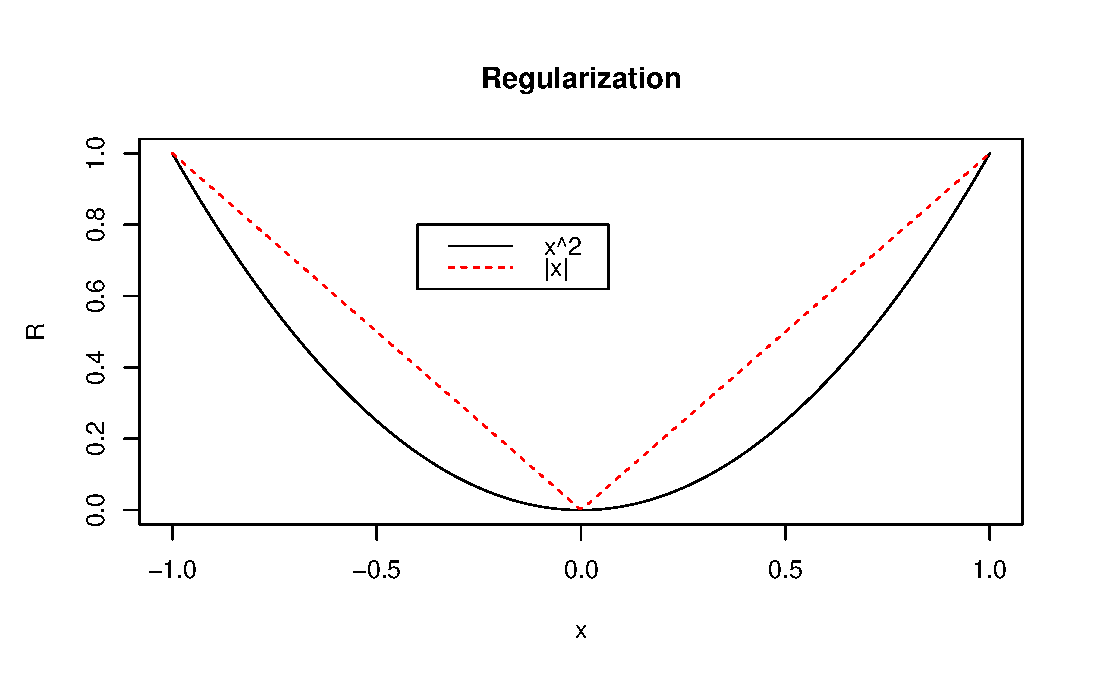
\includegraphics[width=6in]{04SelfTaught/L1L2Norm.eps}
\end{center}
\caption{เปรียบเทียบค่า $x^2$ กับ $|x|$ ในช่วง $x \in [-1,1]$}
\label{fig: deep L1 L2 Norm}
\end{figure}
%

\paragraph{ตัวอย่าง}
รายนะและคณะได้แสดงตัวอย่างของเบซิส ดังแสดงในรูป~\ref{fig: deep Raina et al Fig 2}.
ภาพซ้าย แสดง ตัวอย่างของเบซิส ที่เรียนจาก image patches (ขนาด $14 \times 14$ pixels) ที่สุ่มออกมาจากภาพทิวทัศน์ต่างๆ.
นั่นคือ ให้ $x_u^{(i)}$ เป็นเวกเตอร์ ค่าของพิกเซล $14 \times 14 = 196$ ค่า.
สังเกตุว่าลักษณะของเบซิสที่ได้ คล้ายกับ เป็น ตัวตรวจจับขอบต่างๆที่ผสมเป็นภาพ (edge detection).
ในภาพแสดง เบซิส 32 ตัว: $b_1, b_2, \ldots, b_{32}$ โดยที่ เบซิสแต่ละตัวเป็นเวกเตอร์ขนาด $196$.
ภาพขวา แสดง ตัวอย่างของเบซิส 4 ตัว ที่เรียนจาก sound samples (ขนาด 25 ms) ที่สุ่มมาจากสัญญาณเสียง.
ลักษณะของเบซิสที่ได้ คล้ายกับ เป็น ตัวตรวจจับความถี่ต่างๆที่ผสมเป็นเสียง.
เราจะได้เบซิสเหล่านี้ออกมาหลังจากขั้นตอนที่หนึ่ง (แก้ปัญหา~\ref{eq: deep self-taught unsupervised stage})

%
\begin{figure}
\begin{center}
\begin{tabular}{cc}
\includegraphics[width=2.5in]{04SelfTaught/RainaEtAlFig2a.png} 
& 
\includegraphics[width=2.5in]{04SelfTaught/RainaEtAlFig2b.png}
\end{tabular} 
\end{center}
\caption{ภาพจาก Raina et al 2007 แสดงตัวอย่าง ของ เบซิส (bases):
ภาพซ้าย เป็น ตัวอย่างของเบซิส 32 ตัว ที่เรียนจาก image patches (ขนาด $14 \times 14$ pixels) ที่สุ่มออกมาจากภาพทิวทัศน์ต่างๆ;
ภาพขวา เป็น ตัวอย่างของเบซิส 4 ตัว ที่เรียนจาก sound samples (ขนาด 25 ms) ที่สุ่มมาจากสัญญาณเสียง}
\label{fig: deep Raina et al Fig 2}
\end{figure}
%

หลังจากขั้นตอนที่สอง เราจะได้ ลักษณะสำคัญ $a^{(i)}$'s ซึ่งคือ การกระตุ้นของลักษณะพื้นฐาน (สมการ~\ref{eq: deep self-taught mapping stage}).
แต่ละค่ากระตุ้น ในเวกเตอร์ลักษณะสำคัญ $a^{(i)} = [a^{(i)}_1, a^{(i)}_2, \ldots, a^{(i)}_M]^T$ จะบอกค่าน้ำหนักของ เบซิส ที่จะมาประกอบ กลับไปเพื่อ แทน อินพุต $x_l^{(i)}$.
รูป~\ref{fig: deep Raina et al Fig 3} แสดง เบซิส 3 ตัว กับ ค่ากระตุ้นของแต่ละตัว เพื่อประกอบกลับเป็น อินพุต $x_l^{(i)}$ (โดยประมาณ):
$a_{142}^{(i)} = 0.6$, $a_{381}^{(i)} = 0.8$, $a_{497}^{(i)} = 0.4$ หรือ 
\begin{eqnarray}
a^{(i)} = 
[0, \ldots 0, 0.6, 0, \ldots, 0, 0.8, 0, \ldots, 0, 0.4, 0, \ldots, 0]^T
\nonumber .
\end{eqnarray}
สังเกตุ การกระตุ้น $a^{(i)}$ (ซึ่งคือ ``ลักษณะสำคัญของอินพุตตัวที่ $i$'') มีค่าหร็อมแหร็ม: มีค่ามากๆอยู่ไม่กี่ค่า ค่าการกระตุ้นส่วนใหญ่เป็น $0$.
นี่คือ การที่ การกระตุ้น $a^{(i)}$ สามารถเลือกลักษณะพื้นฐานที่สำคัญของอินพุต $i$ ออกมาได้.
ในลักษณะเดียวกับ ที่เราจำใบหน้าคนจากลักษณะพื้นฐานที่สำคัญ เช่น ตา หู จมูก ปาก โดยละรายละเอียดปลีกย่อยอื่นๆทิ้งไป.
%
ดังนั้น เราอาจมอง การกระตุ้น $a^{(i)}$ นี้ได้ว่า เป็นเสมือนกับ การแทนอินพุต $i$ ในระดับที่สูงขึ้น (higher level representation) หรือ การสรุปย่อ (abstract) ของอินพุต $i$.
และ เราก็จะสามารถใช้ $a^{(i)}$ ไปเป็นอินพุต ของอัลกอริทึ่มเพื่อจำแนกกลุ่ม เช่น SVM หรือ โครงข่ายประสาทเทียม ได้ต่อไป.

%
\begin{figure}
\begin{center}
\includegraphics[width=5in]{04SelfTaught/RainaEtAlFig3.png}
\end{center}
\caption{ภาพจาก รายนะและคณะ 2007; 
อินพุตแต่ละตัว สามารถถูกประมาณได้ด้วย ผลรวมของลักษณะพื้นฐานตามค่าน้ำหนัก;
ลักษณะพื้นฐาน (เบซิส) จะใช้ร่วมกันสำหรับ อินพุตทุกตัว;
แต่ค่าน้ำหนักที่ต่างกันของเบซิสต่างๆ จะผสม ค่าประมาณออกมาให้คล้ายกับอินพุตแต่ละตัว;
อินพุต $x^{(i)}$ แต่ละตัว  จะมี ชุดของค่าน้ำหนักเฉพาะ ของตัวเอง;
ชุดของค่าน้ำหนัก สำหรับ อินพุต $x^{(i)}$ คือ การกระตุ้น $a^{(i)}$.}
\label{fig: deep Raina et al Fig 3}
\end{figure}
%

\begin{minipage}{5.5in}
{\small
\begin{shaded}
สังเกตุว่า แทนที่จะ แปลงรูปขนาดใหญ่ เป็น เบซิส และ ค่าน้ำหนัก โดยตรง, 
รายนะและคณะ สุ่มรูปย่อย (image patches) ที่แต่ละรูปที่ขนาดเท่ากัน และ หาค่า เบซิส และ ค่าน้ำหนัก จาก รูปย่อยเหล่านี้แทน.
วิธีนี้เป็นวิธีที่นิยมมาก ในงาน computer vision เพราะ จะช่วยให้ เราสามารถ จำแนก วัตถุเดียวกัน ที่อยู่ตำแหน่งต่างกันในภาพได้.

หลังจากได้ เบซิส แล้ว, ค่าน้ำหนัก ที่จะใช้ อธิบายภาพใหญ่ จะได้จากทำเทคนิค sliding window,
ที่เราจะหยิบ ส่วนของภาพใหญ่ ที่มีขนาดเท่ากับ image patch ออกมา และ หาค่าน้ำหนักของเบซิสต่างๆที่ ส่วนนั้น จากนั้นก็ขยับไปหยิบส่วนข้างๆ ทำไปจนครบทั้งภาพ\footnote{
การขยับไปส่วนข้างๆ อาจขยับไปทีละพิกเซล หรือ ขยับด้วยก้าวที่หยาบกว่าก็ได้ ขึ้นกับ ประเภทของงาน และ ทรัพยากรที่สนับสนุน.
การขยับไปทีละพิกเซล อาจจะให้ผลที่ดีที่สุด ละเอียดที่สุด แต่ก็จะทำให้ได้ ค่าน้ำหนักเป็นจำนวนมาก ซึ่ง ก็จะเปลืองทรัพยากรการคำนวณ ทั้งเวลา และ หน่วยความจำ.
}.
และ ค่าน้ำหนักของเบซิสต่างๆ ที่ส่วนต่างๆของภาพ จะเป็นลักษณะที่ใช้บรรยายภาพนั้น และใช้เป็นอินพุต สำหรับ อัลกอริทึ่มเพื่อจำแนกกลุ่ม ต่อไป.

รายนะและคณะ กล่าวถึง การใช้ขั้นตอนพิเศษ เพื่อช่วยจัดการทรัพยากรการคำนวณได้มีประสิทธิภาพมากขึ้น, สำหรับรายละเอียด แนะนำให้ศึกษาโดยตรงจาก \cite{RainaEtAl2007a}.

รูป~\ref{fig: deep Raina et al Fig 4} แสดงค่าน้ำหนักของเบซิสต่างๆ ($4$ เบซิส) ที่ส่วนต่างๆของภาพใหญ่: แต่ละค่าพิกเซลในรูปขวามือ คือ ค่าน้ำหนักของเบซิสนั้นที่ส่วนนั้นของภาพ.
พิกเซลสีขาว แทน ค่าน้ำหนักที่เป็นบวกมากๆ และ พิกเซลสีดำ แทน ค่าน้ำหนักที่เป็นลบมากๆ.
จะเห็นว่า ค่าน้ำหนักที่ได้ จะเสมือนเป็น ตัวตรวจจับ ลักษณะของส่วนของภาพที่ใกล้กับเบซิสนั้นๆ.

\end{shaded}
}

\end{minipage}

%
\begin{figure}
\begin{center}
\includegraphics[width=5in]{04SelfTaught/RainaEtAlFig4.png}
\end{center}
\caption{ภาพจาก รายนะและคณะ 2007 (ควรดูเป็นภาพสี); ซ้ายมือ เป็น ภาพใหญ่ต้นฉบับ ของ ตุ่นปากเป็ด; ขวามือ เป็น ค่าน้ำหนักของเบซิสต่างๆที่ได้จากตำแหน่งต่างๆของภาพตุ่นปากเป็ด โดยมีภาพขยายของเบซิสแสดงอยู่ทางซ้าย (ไอคอนเล็กๆ); ค่าน้ำหนักที่ได้เรียงตามตำแหน่งที่ได้จากภาพต้นฉบับ โดย สีพิกเซลขาว แทนค่าน้ำหนักที่เป็นบวกมาก และ สีดำแสดงค่าเป็นลบมาก; สังเกตุว่าค่านำ้หนักที่ได้ ทำตัวเสมือนเป็น การตรวจจับลักษณะของภาพที่ตำแหน่งนั้นๆที่ใกล้เคียงกับเบซิส}
\label{fig: deep Raina et al Fig 4}
\end{figure}
%


ตาราง~\ref{tbl: deep Raina et al 2007 results} นำตัวอย่างผลประเมินของวิธีการเรียนรู้แบบสอนตนเอง จากงานของ รายนะและคณะ 2007\cite{RainaEtAl2007a} มาแสดง.
รายนะและคณะใช้ PCA (Principle Component Analysis) ซึ่งเป็น วิธีดั้งเดิมและยังเป็นที่นิยม ใช้สำหรับการ แปลงอินพุต ไปสู่ ลักษณะสำคัญ มาเพื่อเปรียบเทียบ.
ในตาราง, Unlabeled SC หมายถึง การใช้การเรียนรู้แบบสอนตนเอง และ ใช้ข้อมูลที่ไม่มีฉลาก มาประกอบ; Labeled PCA หมายถึง การใช้ PCA กับเฉพาะอินพุตของข้อมูลที่มีฉลาก;
และ Labeled SC หมายถึง การใช้การเรียนรู้แบบสอนตนเอง แต่ใช้เพียง ข้อมูลที่มีฉลากเท่านั้น.
ในตารางนำผลการประเมินจากงาน 4 อย่าง: (1) Handwritten character recognition ที่จำแนก ค่าความเข้มของพิกเซลทั้ง $28 \times 28$ พิกเซล เป็นตัวอักษร `a' ถึง `z' โดยใช้ ภาพลายมือเขียนของตัวอักษร `a' ถึง `z' เป็น ข้อมูลฝึกที่มีฉลาก และ ใช้ ภาพของลายมือเขียนตัวเลข `0' ถึง `9' เป็นข้อมูลที่ไม่มีฉลาก;
(2) Font character recognition ที่จำแนก ค่าความเข้มของพิกเซลทั้ง $28 \times 28$ พิกเซล เป็นตัวอักษร `a'/`A' ถึง `z'/`Z'
โดยใช้ ภาพฟอนต์ของ ตัวอักษร `a'/`A' ถึง `z'/`Z' เป็นข้อมูลฝึกที่มีฉลาก และ ใช้
ภาพของลายมือเขียนตัวอักษร `a' ถึง `z' เป็นข้อมูลที่ไม่มีฉลาก;
(3) Webpage classication จำแนก bag-of-words\footnote{วิธี bag-of-words เป็น รูปแบบ การแทน ข้อความ ด้วยค่าความถี่ของคำที่พบในบทความ ซึ่งเป็นวิธีหนึ่งที่นิยมใช้ศาสตร์การประมวลผลภาษาธรรมชาติ (natural language processing)} ของหน้าเวป ไปเป็น ประเภทของเวป
โดยใช้ หน้าเวปที่มีการจำแนกประเภทแล้ว เป็น ข้อมูลฝึกที่มีฉลาก
และใช้ บทความข่าว จาก Reuters newswire เป็นข้อมูลที่ไม่มีฉลาก;
และ (4) UseNet article classification จำแนก bag-of-words ของ UseNet posts ไปเป็น ประเภทของโพสต์
โดยใช้ UseNet Posts ที่มีการจำแนกประเภทแล้ว เป็น ข้อมูลฝึกที่มีฉลาก
และใช้ บทความข่าว จาก Reuters newswire เป็นข้อมูลที่ไม่มีฉลาก.

จากผลที่นำเสนอ จะเห็นว่า เมื่อจำนวนข้อมูลที่ใช้ฝึก อัลกอริทึ่มเพื่อจำแนกกลุ่ม มีจำนวนน้อยๆ, Unlabeled SC (การใช้การเรียนรู้แบบสอนตนเอง ประกอบการใช้ข้อมูลที่ไม่มีฉลาก) ช่วยให้ได้ผลการจำแนกที่ดีกว่า การใช้ PCA หรือ การเรียนรู้แบบสอนตนเองแต่ใช้เฉพาะข้อมูลที่มีฉลาก.
แต่เมื่อปริมาณข้อมูลมีมากขึ้น เช่น กรณี งานจำแนก รายมือเขียนตัวอักษร (Handwritten characters) กับข้อมูลฝึก 5000 ตัวอย่าง, 
ผลประโยชน์จากการใช้ ข้อมูลไม่มีฉลาก อาจเห็นไม่ชัดนัก.
ซึ่งเรื่องนี้ ก็สมเหตุสมผลดีที่ว่า หากเรามีข้อมูลสำหรับการฝึกมากพอ เราก็ไม่จำเป็นต้องใช้ ข้อมูลที่ไม่มีฉลากมาช่วย.
งานอื่นๆ ที่แสดงในตาราง อาจไม่ได้มีจำนวนข้อมูลฝึกมากพอจะทำเห็นแนวโน้มในแบบเดียวกัน.
%
สุดท้ายแล้ว การประเมินได้แสดงให้เห็นว่า การเรียนรู้แบบสอนตนเอง สามารถ ใช้ประโยชน์จาก ข้อมูลที่ไม่มีฉลาก เพื่อ เสริม ประสิทธิภาพ การทำงาน ของ การเรียนรู้แบบมีผู้สอนได้ โดยเฉพาะเมื่อ ปริมาณข้อมูลสำหรับฝึกมีน้อย.

%
\begin{table}[hbtp]
\caption{Accuracy on the self-taught learning tasks (ตารางที่ 7 ใน Raina et al 2007)}
\begin{center}
\begin{tabular}{|c|c|c|c|c|}
\hline
Domain & Training & Unlabled & \multicolumn{2}{c|}{Labeld} \\
\cline{4-5}
       & set size & SC       & PCA  & SC \\
\hline
              & 100  & 39.7\% & 36.2\% & 31.4\% \\
Handwritten   & 500  & 58.5\% & 50.4\% & 50.8\% \\
characters    & 1000 & 65.3\% & 62.5\% & 61.3\% \\
              & 5000 & 73.1\% & 73.5\% & 73.0\% \\
\hline
Font          & 100  & 7.0\%  & 5.2\%  & 5.1\% \\
characters    & 500  & 16.6\% & 11.7\% & 14.7\% \\
              & 1000 & 23.2\% & 19.0\% & 22.3\% \\
\hline
              & 4    & 64.3\% & 55.9\% & 53.6\% \\
Webpages      & 10   & 75.9\% & 57.0\% & 54.8\% \\
              & 20   & 80.4\% & 62.9\% & 60.5\% \\
\hline
UseNet 	      & 4    & 63.8\% & 60.5\% & 50.9\% \\
              & 10   & 68.7\% & 67.9\% & 60.8\% \\
\hline
\end{tabular} 
\end{center}
\label{tbl: deep Raina et al 2007 results}
\end{table}

%%%%%%%%%%%%%%%%%%%%%%%%%%%%%%%%%%%%%%%%%%%%%
\begin{minipage}{5.5in}
{\small
\begin{shaded}
การหาค่าดีที่สุด ในปัญหาที่มีข้อกำจัด (Constraint Optimization)
\index{constraint optimization}
\index{soft constraint}
\index{hard constraint}
\\
นิพจน์~\ref{eq: deep self-taught unsupervised stage} มี ข้อกำจัดของการหาค่าดีที่สุดอยู่.
ด้วยเหตุผล ตามจุดประสงค์ การเรียนรู้ลักษณะสำคัญ, เราอาจไม่จำเป็นต้องบังคับ ข้อจำกัด
$\| b_j \|_2 \leq 1, \forall j \in 1, \ldots, M$ อย่างเข้มงวดก็ได้. นั่นคือ,เราสามารถทำ soft constraint ได้.
เช่น แทนการแก้ปัญหาตาม นิพจน์~\ref{eq: deep self-taught unsupervised stage}, เราอาจเพียงเลือกทำ
\begin{eqnarray}
  \min_{b,a} & \sum_i \| x_u^{(i)} - \sum_j a_j^{(i)} b_j \|_2^2 + \beta \| a^{(i)} \|_1
%\nonumber \\
  + \gamma \cdot \sum_{j=1}^M \{ P(\| b_j \|_2 - 1) \}^2
\label{eq: deep self-taught penalty}  
\end{eqnarray} 
เมื่อ
\begin{eqnarray}
P(m) = \left\{\begin{matrix}
m & \mbox{ for } m > 0 \\
0   & \mbox{ for } m \leq 0
\end{matrix} \right.
\nonumber
\end{eqnarray}
และ เลือกค่า $\gamma$ ให้ใหญ่เพียงพอ.

แต่หากเราต้องการบังคับข้อจำกัดอย่างเข้มงวด (hard constraint), เราอาจเลือกใช้ วิธีการลงโทษ (Penalty Method) \index{Penalty Method} จากศาสตร์ของ การหาค่าดีที่สุด ในปัญหาที่มีข้อกำจัด (Constraint Optimization)\footnote{
ดู \cite{ChongZak2ndEd} สำหรับรายละเอียด.}
มาช่วยได้.
วิธีการลงโทษ จะแก้ปัญหา~\ref{eq: deep self-taught penalty} โดยเริ่มจากค่า $\gamma$ น้อยๆ และ ค่อยๆเพิ่มค่า $\gamma$ และแก้ปัญหาใหม่, สังเกตุผลลัพธ์ที่ได้ ต่อ ค่า $\gamma$ ที่เพิ่มขึ้น;
จนกระทั่ง ผลลัพธ์ลู่เข้า (convergence) และค่าที่ผลลัพธ์ลู่เข้าหา คือ คำตอบของปัญหาที่บังคับข้อจำกัดอย่างเข้มงวด.
\end{shaded}
}
\end{minipage}
%%%%%%%%%%%%%%%%%%%%%%%%%%%%%%%%%%%%%%%%%%%%%

\section{การเรียนรู้แบบลึก}
\label{deep learning: deep learning}

(จาก Introduction to Deep Learning Algorithm, Y. Bengio, Notes de cours IFT6266 Hiver 2010, \url{http://www.iro.unmontreal.ca/~pift6266/H10/notes/deepintro.html})

%
\begin{SCfigure}
\centering

\includegraphics[width=1.5in]{04ANNDeep/ShallowStructure.png}
\label{fig: deep shallow structure}

\caption{ภาพแสดง การใช้งานโครงสร้างแบบตื้น กับ งานการเรียนรู้แบบมีผู้สอน.
  ในรูปแสดง โครงข่ายประสาทเทียม 1 ชั้นซ่อน หรือ โครงข่ายความลึก 2 ชั้น (มีค่าน้ำหนัก 2 ชุด)}

\end{SCfigure}
%

โครงข่ายประสาทเทียม ความลึก $2$ ชั้น นั้น ทางทฤษฎี บอกว่า สามารถแทน ฟังชั่นใดๆก็ได้ ที่ความแม่นยำที่ต้องการ เพียงให้มีจำนวนหน่วยในชั้นซ่อนมากพอ\cite{Cybenko1989a, Hornik1991a, Bishop2006a}[ทฤษฎี Universal Approximator].
แต่ สำหรับ ฟังชั่นที่ซับซ้อนและมีการแปรผันสูงมากๆ\footnote{
การแปรผันสูง นี้ไม่ได้หมายถึงการแปรผันสูงในทางสถิติ แต่เป็นการแปรผันสูงในลักษณะความสัมพันธ์ระหว่างอินพุตและเอาต์พุต เช่น ค่าอินพุต เปลี่ยนแปลงเพียงเล็กน้อย ก็มีผลต่อค่าเอาต์พุต มาก.
} (ปัญหาที่ยาก), จำนวนหน่วยในชั้นซ่อน ของ โครงข่ายประสาทเทียม ความลึก $2$ ชั้น ที่ต้องใช้ อาจจะมากมหาศาล (จนเป็น อุปสรรคสำคัญ ในทางปฏิบัติ).
มีฟังชั่นหลายแบบที่สามารถประมาณได้อย่างมีประสิทธิภาพ ด้วย โครงข่ายประสาทเทียมที่มีความลึกมาก,
แต่ไม่สามารถทำได้อย่างมีประสิทธิภาพ กับโครงข่ายประสาทเทียมที่ตื้น\footnote{
ปัจจุบัน ผู้เขียนยังไม่พบนิยาม หรือ ขอบเขตที่แน่ชัดที่แบ่งระหว่าง โครงสร้างที่ลึก และ โครงสร้างที่ตื้น.
เพียงแต่ ความเข้าใจทั่วไป คือ โครงข่ายประสาทเทียม ความลึก $2$ ชั้น เป็น โครงสร้างแบบตื้น.)
}.

รูป~\ref{fig: deep shallow structure} และ~\ref{fig: deep deep structure} เปรียบเทียบโครงสร้างแบบตื้นและแบบลึก.
โครงสร้างในรูป~\ref{fig: deep shallow structure} มีชั้นซ่อนหนึ่งชั้น. โครงข่ายประสาทเทียมแบบจ่ายไปข้างหน้าที่มีชั้นซ่อนหนึ่งชั้นแบบนี้ จะมี ค่าน้ำหนัก $2$ ชุด: $W^{(1)}$ และ $W^{(2)}$.
โดย $W^{(1)}$ มี ค่าน้ำหนักทั้งหมด $M_1 \times (1 + M_0)$ ค่า, เมื่อ $M_0$ คือ จำนวนมิติของอินพุต และ $M_1$ คือ จำนวนหน่วยซ่อนในชั้น)
และ $W^{(2)}$ มี ค่าน้ำหนักทั้งหมด $M_2 \times (1 + M_1)$ ค่า, เมื่อ $M_2$ คือ จำนวนมิติของเอาต์พุต.
ดังนั้นหาก อินพุตมี $3$ มิติ, จำนวนหน่วยซ่อนในชั้น เป็น $12$, และ เอาต์พุตมี 2 มิติ ดังในรูป~\ref{fig: deep shallow structure}, 
โครงข่ายประสาทเทียมแบบจ่ายไปข้างหน้านี้ จะมีจำนวนพารามิเตอร์ เป็น $(12 \times 4) + (3 \times 13) = 87$ ค่า.
โครงสร้างในรูป~\ref{fig: deep deep structure} มี $3$ ชั้นซ่อน.
ในบริบทเดียวกัน, มีค่าน้ำหนัก $4$ ชุด: $W^{(1)}$, $W^{(2)}$, $W^{(3)}$, และ $W^{(4)}$.
หากจำนวนหน่วยซ่อนในแต่ละชั้น เป็น $4$ ทั้งหมด (จำนวน หน่วยซ่อนรวม เป็น $12$ เท่ากับ จำนวนรวม ในรูป~\ref{fig: deep shallow structure}), 
แต่ จำนวนพารามิเตอร์ เป็น $(4 \times 4) + (4 \times 5) + (4 \times 5) + (3 \times 5) = 71$ ค่า\footnote{
ตัวอย่างนี้ เพียงเพื่อ ชี้ให้เห็น มุมมองของการคิดจำนวนพารามิเตอร์เท่านั้น.
การประเมิน ความสามารถในการประมาณฟังชั่น (representative power) ของโมเดล ต่อ จำนวนพารามิเตอร์ จะซับซ้อนกว่านี้, ขึ้นกับรายละเอียดและสถานะการณ์ และ อาจต้องการ การทดลอง ประกอบ.
}.
แม้จำนวนหน่วยคำนวณย่อยรวมจะเท่ากัน แต่การจัดโครงสร้างเป็นแบบลึก ช่วยให้จำนวน พารามิเตอร์รวมน้อยกว่า.
ซึ่งในการคำนวณจริง จำนวนพารามิเตอร์รวมที่น้อยกว่า ทำให้การคำนวณโดยรวมน้อยลง\footnote{
หมายเหตุ การใช้โครงสร้างที่ลึกเกินไป ก็อาจทำให้ได้ผลแย่ลงได้ (ดูแบบฝึกหัดข้อ 8)
} เช่น การคำนวณ เกรเดียนต์ของฟังชั่นจุดประสงค์ ต่อ พารามิเตอร์แต่ละตัว ก็จะน้อยลง.

อาจารย์เบนจิโอ (Bengio) \cite{Bengio2009a}[pp. 8] อธิบายว่า ความลึกของโครงข่าย เชื่อมโยงกับ ความยืดหยุ่นของโมเดล.
%
โดยทั่วไปแล้ว โครงสร้างที่ลึก (deep architectures) จะสามารถ แทน ฟังชั่นที่แปรผันสูง (highly-varying) ได้อย่างกระทัดรัดกว่า โครงสร้างที่ตื้น:
หากใช้ โครงสร้างที่ตื้น (shallow architectures) มาประมาณ ฟังชั่นที่แปรผันสูงเดียวกัน จะต้องการ โครงสร้างตื้นขนาดใหญ่มาก (เช่น หน่วยซ่อนของโครงข่ายขนาด $2$ ชั้น จะต้องการเป็นจำนวนมหาศาล เมื่อเปรียบเทียบกับ จำนวนหน่วยซ่อนรวม หากใช้ โครงข่ายขนาด $>2$ ชั้น).
ตัวอย่างเชิงทฤษฎีและการคำนวณ ที่แสดง ประสิทธิภาพ ของ การใช้โครงสร้างลึก ต่อ การใช้โครงสร้างตื้น ดูได้จาก \cite{Bengio2009a}.
นอกจากนั้น อาจารย์เบนจิโอ กับ อาจารย์เลอคัน (LeCun) \cite{BengioLeCun2007a} อภิปรายว่า 
โครงสร้างตื้น ไม่มีประสิทธิภาพ ในแง่ที่ มันต้องการ หน่วยคำนวณ และ ตัวอย่าง เป็นจำนวนมาก
และ ได้ยกตัวอย่าง เพื่อสนับสนุนข้ออภิปรายนี้ด้วย. 
ตัวอย่าง ของ \cite{BengioLeCun2007a} เปรียบเทียบ การทำงาน ในปัญหาการรู้จำภาพ ของ โครงสร้างแบบตื้น กับ โครงสร้างแบบลึก.
ซึ่งได้ผลสรุปว่า โครงสร้างลึก นอกจากจะให้ผลที่ผิดพลาดน้อยกว่า โครงสร้างตื้นแล้ว,
โครงสร้างลึกยังทำงานได้เร็วกว่า และ สามารถฝึกได้เร็วกว่า สำหรับชุดข้อมูลขนาดใหญ่ อีกด้วย.
อาจารย์เบนจิโอและเลอคัน อธิบายว่า โครงสร้างลึก มีศักยภาพ ในการสรุปความสัมพันธ์ ในแบบไม่ท้องถิ่น.
และ ศักยภาพนี้ เป็นสิ่งที่จำเป็น สำหรับการก้าวหน้า ไปในทิศทาง สำหรับ ปัญหาประดิษฐ์.

\begin{verse}
``We argue that deep architectures have the potential to generalize in non-local ways, i.e., beyond immediate neighbors, and that this is crucial in order to make progress on the kind of complex tasks required for artificial intelligence.''
\\Bengio และ LeCun\cite{BengioLeCun2007a} 
\end{verse}

%
\begin{figure}
\begin{center}
\includegraphics[width=4in]{04ANNDeep/DeepStructure.png}
\end{center}
\caption{ภาพแสดงโครงสร้างแบบลึก เปรียบเทียบกับ รูป~\ref{fig: deep shallow structure}.
  ในภาพเป็นโครงสร้างที่มี 3 ชั้นซ่อน (4-layer network).}
\label{fig: deep deep structure}
\index{deep learning}
\end{figure}
%

นอกจากมุมมองทางทฤษฎีแล้ว มุมมองจากแรงบันดาลใจของระบบธรรมชาติ ก็สนับสนุนแนวคิดของ โครงสร้างลึก.

โครงสร้างและการเชื่อมต่อ ของระบบสมองของมนุษย์ ก็มีลักษณะเป็นโครงสร้างแบบลึก.
ตัวอย่าง เช่น visual cortex \cite{NeuroscienceOnline}[Chapter 15] ที่มี สัญญาณ จากประสาทตา ผ่านไปที่ lateral geniculate nucleus (LGN).
สัญญาณจาก LGN ส่งผ่านไปที่ คอร์เทกซ์สายตา (visual cortex) ใน เขตสายตา V1 ซึ่งนับเป็นจุดเริ่มต้น การประมวลผลและรับรู้ภาพ.

นอกจากนั้น การรับรู้ของมนุษย์ ดูเหมือนจะมาจากโครงสร้างแบบลึก.
มนุษย์เรา จัดเรียงความคิดและการรับรู้ต่างๆ เป็นแบบลำดับชั้น:
เราใช้การรับรู้แบบลำดับชั้น (hierarchical perception) เช่น เรารับรู้ว่า บีเกิล เป็นพันธ์ุหมา; หมา เป็น สัตว์เลี้ยงลูกด้วยนม; และ สัตว์เลี้ยงลูกด้วยนม เป็น สิ่งมีชีวิต เป็นต้น.
มนุษย์เรา เริ่มเรียนรู้จากเรื่องง่ายๆ แล้วค่อยๆต่อยอด เพิ่มเติม เพื่อทำความเข้าใจ หรือ เพื่อ อธิบายเป็นเรื่องที่ซับซ้อนขึ้น.
วิศวกรเองก็ใช้แนวคิดของ multiple levels of abstraction ในการแตกปัญหาและวิธีแก้ เป็นปัญหาย่อยๆ.

โครงสร้างแบบลึก เป็นแนวทางหนึ่ง ที่ทำให้ เราสามารถเพิ่ม การเรียนรู้แบบเป็นลำดับชั้นนี้เข้าไปได้.
การเรียนรู้แบบเป็นลำดับชั้น เชื่อมโยงอย่างมาก กับแนวคิดของการเรียนรู้เชิงโยกย้าย และ การใช้ประโยชน์จากข้อมูลที่ไม่มีฉลาก ในงานจำแนกข้อมูล.
แนวคิด ของ การเรียนรู้เชิงโยกย้าย (transfer learning) คือ การที่เราเรียนรู้ที่จะทำงานได้ดีสำหรับงานหนึ่งแล้ว เราน่าจะเรียนรู้งานใหม่(ที่มีลักษณะใกล้เคียงกับงานเดิม)ได้ดีขึ้น.
หรือ เรียกง่ายๆว่า ใช้ประโยชน์จากพื้นความรู้เดิม เช่น การสอนการโต้คลื่น กับ คนที่ว่ายน้ำเป็นแล้ว น่าจะง่ายกว่า สอนกับคนที่ว่ายน้ำไม่เป็นเลย.
%
การใช้โครงสร้างแบบลึก ยังสามารถช่วยการทำการเรียนรู้เชิงโยกย้าย ได้อย่างมีประสิทธิภาพมากขึ้นอีกด้วย ดังอภิปรายในหัวข้อ~\ref{deep learning: self-taught learning}.

งานจำแนกข้อมูล เป็นงานการเรียนรู้แบบมีผู้สอน ซึ่ง เราต้องการตัวอย่างข้อมูล พร้อมฉลาก เพื่อฝึกโครงข่ายประสาทเทียม.
แต่ ในทางปฎิบัติแล้ว ปัญหาหลายอย่าง ข้อมูลที่มีฉลากหาได้ยาก ในขณะที่ ข้อมูลที่ไม่มีฉลาก สามารถหาได้ง่ายกว่ามาก.
ตัวอย่างเช่น งานรู้จำวัตถุ (object recognition) ซึ่งจุดประสงค์ คือ การระบุชนิดของวัตถุในภาพ.
การหาภาพทำได้ง่าย 
แต่ การหาภาพพร้อมฉลากที่ถูกต้อง ที่จะสามารถนำมาใช้ ฝึกโครงข่ายประสาทเทียมแบบมีผู้สอนนั้น ไม่ง่ายนัก.
โครงสร้างแบบลึก ยังสามารถช่วยให้เราใช้ประโยชน์ จากข้อมูลที่ไม่มีฉลาก มาเสริมการฝึกโครงข่ายประสาทเทียมแบบมีผู้สอน ได้อีกด้วย.

สรุปโดยย่อ ปัจจัยหลักๆที่ จูงใจ การใช้โครงสร้างแบบลึก มีดังนี้
\begin{itemize}
\item สามารถใช้ จำนวนรวม ของ หน่วยคำนวณ ที่น้อยกว่า โครงสร้างแบบตื้น ในการประมาณความสัมพันธ์ ที่ซับซ้อนและแปรผันสูงมาก ได้.
\item โครงสร้างทางประสาท ในธรรมชาติ มีลักษณะเป็นโครงสร้างแบบลึก.
\item โครงสร้างแบบลึก อนุญาติให้ โครงข่ายประสาทเทียม สามารถมี คุณสมบัติ hierarchical perceptions และ multiple levels of abstraction ซึ่งเป็นพื้นฐาน ของ กระบวนการคิด รับรู้ และ แก้ปัญหา ของมนุษย์ ได้.
\item โครงสร้างแบบลึก อนุญาติให้ เราสามารถใช้ ข้อมูลที่ไม่มีฉลาก (unlabeled data) มาช่วยปรับปรุง คุณภาพของการทำงานแบบมีผู้สอนได้.
ข้อมูลที่ไม่มีฉลาก สามารถหาได้ง่าย และ มีต้นทุน ต่ำกว่า การหาข้อมูลที่มีฉลาก.
\item โครงสร้างแบบลึก ยังช่วยให้การทำ การโยกย้ายการเรียนรู้ (transfer learning) ทำได้อย่างมีประสิทธิผลมากขึ้น.
\end{itemize}

ถึงแม้จะมีปัจจัยต่างๆที่ ชี้ประโยชน์ของการใช้โครงสร้างแบบลึก.
แต่อย่างไรก็ตาม การฝึกโครงสร้างแบบลึกทำได้ยากมาก จนกระทั่งช่วงปี ค.ศ. 2006 ที่ อาจารย์เจฟฟรีย์ ฮินตันและคณะ \cite{HintonEtAl2006a} เผยแพร่ ผลงานสำคัญ ที่เป็นเสมือนหลักไมล์ ของ ศาสตร์การเรียนรู้ของเครื่อง และ เป็น งานที่กระตุ้น การศึกษาวิจัย การเรียนรู้เชิงลึก จนทำให้เกิดการประยุกต์ใช้อย่างกว้างขวางต่อมา.
% การศึกษาเรื่อง Deep Belief Networks (DBN) ของ เจฟฟรีย์ ฮินตัน (Geoffrey Hinton)
%\begin{itemize}
%\item Hinton, G. E., Osindero, S. and Teh, Y., A fast learning algorithm for deep belief nets, Neural Computation 18: 1527-1554, 2006.
%\item Yoshua Bengio, Pascal Lamblin, Dan Popovici and Hugo Larochelle, Greedy Layer-Wise Training of Deep Networks, in J. Platt et al (Eds), Advances in Neural Information Processing Systems 19 (NIPS 2006), pp. 153-160, MIT Press, 2007.
%\item Marc'Aurelio Ranzato, Christopher Poultney, Sumit Chopra and Yann LeCun, Efficient Learning of Sparse Representations with an Energy-Based Model, in J. Platt et al. (Eds), Advances in Neural Information Processing Systems (NIPS 2006), MIT Press, 2007.
%\end{itemize}
%

โดย อาจารย์เจฟฟรีย์ ฮินตันและคณะ \cite{HintonEtAl2006a} ใช้ Deep Belief Networks (DBNs) ที่ใช้ Restricted Boltzmann Machines (RBMs) ในการทำการเรียนรู้แบบไม่มีผู้สอน เพื่อเรียน representations ของแต่ละชั้นซ่อน;
ต่อมา ทีมของอาจารย์เบนจิโอ \cite{BengioEtAl2007a} ศึกษา และเปรียบเทียบการใช้ RBMs กับ auto-encoders;
ส่วน ทีมของอาจารย์รานซาโต \cite{RanzatoEtAl2007a} ใช้ sparse auto-encoder กับบริบทของ convolution architecture.
ทั้ง 3 แนวทาง (RBMs, autoencoders, และ convolution networks) เป็น แนวทางหลักๆ ของการศาสตร์การเรียนรู้เชิงลึก ในช่วงเริ่มต้น.

หลักการที่สำคัญ ซึ่งพบในทุกๆงานเหล่านี้ ก็คือ:
\begin{itemize}
\item ใช้การเรียนรู้แบบไม่มีผู้สอน (unsupervised learning) เพื่อเรียน ลักษณะที่สำคัญ (representations) ของอินพุต ซึ่ง เท่ากับเป็น การปรับค่าน้ำหนักเริ่มต้น ให้กับ แต่ละชั้นซ่อน ของโครงสร้างแบบลึก.
\item ทำการเรียนรู้แบบไม่มีผู้สอนไปทีละชั้นซ่อน โดยเริ่มจากอินพุต ขยับไป ทางเอาต์พุต และใช้ ลักษณะสำคัญที่เรียนได้ ในแต่ละชั้น ไปใช้เป็น อินพุต สำหรับชั้นถัดไป.
ขั้นตอนการใช้ การเรียนรู้แบบไม่มีผู้สอน เพื่อช่วยหาค่าน้ำหนักเริ่มต้น แบบนี้ จะเรียกว่า การทำ พรีเทรน (pre-train).
\index{pre-train}
\item ขั้นตอนสุดท้าย คือ จะใช้การเรียนรู้แบบมีผู้สอน เพื่อ ปรับค่าน้ำหนักของทุกๆชั้นอย่างละเอียดอีกที รวมถึง การมีชั้นสุดท้าย เพิ่มขึ้นมา เพื่อให้โครงข่ายประสาทเทียม ทำงานทำนายแบบที่ต้องการ.
\end{itemize}

%รวมถึง การใช้ฟังชั่นการกระตุ้นประกอบกับเรกูลาไรเซชั่นแบบใหม่, การมีข้อมูลเป็นจำนวนมาก, และ การมีทรัพยากรคำนวณที่มีสมถนะสูง เป็น

อย่างไรก็ตาม งานศึกษาโครงสร้างแบบลึกในช่วงหลัง มีการนำเอาฟังชั่นค่ากระตุ้น ได้แก่ เรคติไฟด์ลิเนียร์ (rectified linear) \index{rectified linear} \index{เรคติไฟด์ลิเนียร์} มาใช้แทนซิกมอยด์ฟังชั่น ประกอบกับ การทำเรกูลาไรเซชั่น ด้วยวิธี ดรอปเอาต์ (dropout) \index{dropout} \index{ดรอปเอาต์} ซึ่งพบว่า ทำให้สามารถฝึกโครงข่ายได้ง่ายขึ้น.
จนกระทั่ง พบว่า หากมี ข้อมูลที่มีฉลาก เป็นจำนวนมาก, การฝึกโครงสร้างแบบลึก ก็สามารถทำได้ดี แม้ไม่ได้ทำ การปรับน้ำหนักค่าเริ่มต้นก่อน:
กล่าวคือ งานการเรียนรู้แบบลึกในช่วงหลัง พบว่า หากจำนวนข้อมูลมีมากพอ, เราสามารถใช้ โครงสร้างแบบลึก เรียนรู้งานแบบมีผู้สอนได้เลย โดย แม้แต่จะใช้ค่าน้ำหนักเริ่มต้นด้วยการสุ่ม (ไม่ต้องทำ pre-train).
นอกจากนั้น ทรัพยากรด้านการคำนวณสมถะสูง ก็เป็นอีกปัจจัยที่ทำให้การฝึกโครงข่ายแบบลึกขนาดใหญ่สามารถทำได้ดี ดังเช่น งานการจำแนกลายมือเขียน ของ (? cite Cira..? See MNIST for reference).

เนื้อหาของการเรียนรู้แบบลึกต่อไปนี้ ผู้เขียนได้รับอิทธิพลหลักมาจาก 
\cite{LarochelleEtAl2007a, Larochelle2013a, Hinton2013a, Ng2012a}
โดย ผู้เขียนได้ปรับแต่งให้เหมาะสมสำหรับ การแนะนำ การเรียนรู้แบบลึก เบื้องต้น.
ผู้อ่านที่สนใจศึกษาเพิ่มเติม ผู้เขียนแนะนำแหล่งข้อมูลที่อ้างอิงเหล่านี้สำหรับการเริ่มต้น.

BREAK HERE Mar 10th, 2015.

%งานประยุกต์ใช้โครงสร้างแบบลึกในเวลาต่อๆมา พบว่า แม้ไม่ได้ทำ การมีข้อมูลที่มีฉลากเป็นจำนวนมาก รวมถึง ทรัพยากรในการคำนวณ เช่น สมถนะของคอมพิวเตอร์ การนำ GPU มาช่วยประมวลผล 
%ภายหลังจากที่มีการนำฟังชั่นการกระตุ้นแบบใหม่ ได้แก่ rectified linear มาใช้แทนซิกมอยด์ฟังชั่น

ลักษณะสำคัญระดับล่าง (lower-level features) จะค่อยๆถูกรวม เป็น ลักษณะสำคัญระดับสูงขึ้น ($\sim$ แนวคิดที่เป็นนามธรรมมากขึ้น)



\subsection{Sparse Autoencoder}

จาก \cite{ufldl} (Autoencoders and Sparsity), การกระตุ้นเฉลี่ย ของแต่ละหน่วยซ่อน (ของชั้นที่ 1) สามารถวัดได้จาก
\begin{eqnarray}
 \hat{\rho}_m &=& \frac{1}{N} \sum_{n=1}^N h \left( 
w^{(1)}_{m,0} + \sum_{d=1}^D w^{(1)}_{m,d} \cdot x_{d,n} \right)
 \nonumber \\ 
&=& \frac{1}{N} \sum_{n=1}^N h \left( 
 \vec{w}^T_m
  \cdot \begin{bmatrix}
 1 \\
 \vec{x}_n
 \end{bmatrix} \right)
 \nonumber \\ 
&=& \frac{1}{N} \sum_{n=1}^N z_{m,n}
 \nonumber \\  
\label{eq: deep sparse rhohat} 
\end{eqnarray}

เราควบคุมให้ค่าการกระตุ้นเฉลี่ยใกล้เคียงกับค่าเป้าหมาย $\rho$ ได้โดย
\begin{eqnarray}
 \mathrm{Cost} = \mathrm{Cost}_{\mathrm{recon}} 
  + \beta \sum_{m=1}^M \rho \log \frac{\rho}{\hat{\rho}_m} + (1 - \rho) \log \frac{1 - \rho}{1 - \hat{\rho}_m}
\label{eq: deep sparsity cost}  
\end{eqnarray}
เมื่อ $\mathrm{Cost}_{\mathrm{recon}}$ แทน recontruction cost (ค่า cost ในสมการ~\ref{eq: ann cost fn biclass}\footnote{สำหรับอินพุตที่มีค่าอยู่ระหว่าง $[0,1]$.}).
เทอม $\rho \log \frac{\rho}{\hat{\rho}_m} + (1 - \rho) \log \frac{1 - \rho}{1 - \hat{\rho}_m}$ นี้ว่า Kullback-Leibler (KL) divergence\footnote{ทฤษฎีความน่าจะเป็น และ ทฤษฎีสารสนเทศ จะเรียก 
รายละเอียดเกี่ยวกับ KL เทอม ศึกษาเพิ่มเติมได้จาก \cite{KullbackLeibler1951a}.
}.
เทอม KL จะใช้วัดความต่างระหว่างการกระจายความน่าจะเป็นของสองค่า $\rho$ กับ $\hat{\rho}_m$.
รูป .. แสดงค่า KL ที่ค่า $\rho$ และ $\hat{\rho}_m$ ต่างๆ. 
ค่า KL จะเป็น $0$ เมื่อ $\rho = \hat{\rho}_m$ และ ค่า KL มีค่ามาก เมื่อ ค่า $\rho$ และ $\hat{\rho}_m$ ต่างกันมาก.

เมื่อหาค่าอนุพันธ์ ของสมการ~\ref{eq: deep sparsity cost} 
แล้วจะพบว่า เรายังสามารถคำนวณค่าเกรเดียนต์ ด้วยวิธีการแพร่กระจายย้อยกลับ
เมื่อรวมเงื่อนไขบังคับ sparsity เพียงแต่ดัดแปลง สมการ~\ref{eq: ANN BP delta j} ให้เป็น
\begin{eqnarray}
  \delta_j &=& h'(a_j) \left( \sum_k w_{kj} \delta_k + \beta \left( -\frac{\rho}{\hat{\rho}_j} + \frac{1 - \rho}{1 - \hat{\rho}_j} \right) \right)
\nonumber \\
&=& h'(a_j) \sum_k w_{kj} \delta_k + \beta \cdot h'(a_j) \left( -\frac{\rho}{\hat{\rho}_j} + \frac{1 - \rho}{1 - \hat{\rho}_j} \right)
\label{eq: deep BP delta j sparsity}
\end{eqnarray}
เท่านั้น.
% 


%
\begin{figure}
\begin{center}
\includegraphics[width=6in]{04ANNDeep/KL01.eps}
\end{center}
\caption{Kullback-Liebler term ที่ค่าเปรียบเทียบต่างๆ}
\label{fig: deep KL characteristics}
\end{figure}
%



``The restricted Boltzmann machine has been the subject of a recent resurgence of interest due to its role as the building block of the deep belief network. Deep belief networks are designed to learn feature hierarchies to automatically find high-level representations for high-dimensional data. A deep belief network comprises a stack of restricted Boltzmann machines. Given a piece of data (state of the lowest visible variables), each layer's most likely hidden states are treated as data for the next layer. A new effective train methodology for deep belief networks, which begins by training each layer in turn as an RBM using contrastive divergence, was introduced by Hinton et al. \cite{HintonEtAl2006a}. This method led to many new applications in general machine learning problems including object recognition and dimensionality reduction \cite{HintonSalakhutdinov2006a}. ... 
Le Roux and Bengio \cite{LeRouxBengio2008a} showed that any distribution with support on $r$ visible states may be arbitrarily well approximated provided there are at least $r+1$ hidden nodes.
Therefore, any distribution can be approximated with $2^n + 1$ hidden nodes [$n$ is a number of observed variables].

Therefore any distribution can  '' \cite{CuetoEtAl2009a}

``The central hypothesis is that good feature sets contain features that are highly correlated
with the class, yet uncorrelated with each other.'' from Hall, M. A., Correlation-based Feature Selection for Machine Learning, Ph.D. Thesis, Department of Computer Science, University of Waikato, New Zealand, 1999


``One of the main purposes of unsupervised learning is to produce good representation for data, that can be used for detection, recognition, prediction, or visualization. Good representation eliminate irrelevant variabilities of the input data, while preserving the information that is useful for the ultimate task.''
Marc'Aurelio Ranzato, Y-Lan Boureau, Yann LeCun, "Sparse Feature Learning for Deep Belief Networks", 

\section{ศึกษาเพิ่มเติม}

สำหรับภาพรวมของ โครงข่ายประสาทเทียมแบบลึก, ผู้เขียนแนะนำงานของ ชมิดฮูแบร์ และ เติ้งกับหยู \cite{Schmidhuber2015a, DengYu2014a}.

สำหรับ การเรียนรู้ของเครื่อง โดยทั่วไป, 
ปัจจุบัน มี video clips และ online courses เป็นจำนวนมาก.
จากตัวเลือกมากมาย, ผู้เขียนแนะนำ online course: Machine Learning ของ Andrew Ng ที่อยู่บน Coursera.com, ที่หลายๆผู้เชี่ยวชาญหลายๆท่าน ยกให้เป็นแหล่งการเรียนรู้ ศาสตร์การเรียนรู้ของเครื่อง ที่ดีที่สุด แหล่งหนึ่ง.
สำหรับตำรา, ผู้เขียนพบว่ามีตำราเกี่ยวกับการเรียนรู้ของเครื่องที่ดีอยู่เป็นจำนวนมาก แต่ที่ตำราผู้เขียนแนะนำ:
Simon Haykin สำหรับ โครงข่ายประสาทเทียม และ การเรียนรู้ของเครื่อง ทั้งทฤษฎีและข้อแนะนำในทางปฏิบัติ
Bishop สำหรับ การอธิบาย ที่เข้าใจง่าย และ หากให้ประกอบกับ Nabney ที่มีตัวอย่างและโค้ด matlab จะทำให้เข้าใจได้ดีขึ้น
สุดท้าย หากไม่กล่าวถึง Tom Mitchell สำหรับตำรา การเรียนรู้ของเครื่อง ผู้เขียนก็รู้สึกเหมือนยังทำหน้าที่ได้ไม่สมบูรณ์

สำหรับการเรียนรู้แบบเสริมกำลัง (Reinforcement Learning) ซึ่งโดยส่วนตัวแล้ว ผู้เขียนสนใจมาก,
 แต่ด้วยข้อจำกัดของเนื้อหาที่มาก ของการเรียนรู้แบบมีผู้สอน ประกอบกับความซับซ้อนของเนื้อหาของการเรียนรู้แบบเสริมกำลัง, 
ผู้เขียนจึงละเอาไว้สำหรับโอกาสหน้า.
แต่สำหรับ ผู้อ่านที่สนใจผู้เขียนแนะนำ
... Sutton Barto, Powell, Keabling .., My CIE paper, ... all my papers

ความก้าวหน้าล่าสุด ... ICML, NIPS

JMLR, ...

\begin{verse}
``Success is not final, failure is not fatal: \\
it is the courage to continue that counts.'' \\
Winston Churchill
\end{verse}

\section{แบบฝึกหัด}
\label{section: Deep exercises}

\paragraph{1.} 
ออกแบบการทดลอง เพื่อ เปรียบเทียบผลการทำงาน โครงข่ายประสาทเทียมแบบจ่ายไปข้างหน้า $2$, $3$, และ $4$ ชั้น, โดย ใช้การกำหนดค่าเริ่มต้นแบบสุ่ม (ดูบท~\ref{chapter: Applications of ANN}) และ การฝึกโครงข่ายด้วยวิธีการแพร่กระจายย้อยกลับ (อาจจะใช้กับ วิธีลงเกรเดียนต์ หรือ วิธีฝึกที่มีประสิทธิภาพมากขึ้น ก็ได้, ดูบท~\ref{chapter: Suggestions for ANN}).
การทดลองให้ศึกษาผลของการทำงานของโมเดล ต่อ จำนวนข้อมูลที่นำมาฝึกด้วย.
เลือกข้อมูลมาทดลอง, ทำการทดลอง, นำเสนอผล, และ สรุปผล.

\paragraph{2.} 
จากแบบฝึกหัดข้อ 1, อภิปรายว่า ทำไม การฝึกโครงข่ายประสาทเทียมแบบจ่ายไปข้างหน้า ที่ลึกมากๆ ถึงทำได้ยาก และ ผลการฝึกถึงไม่ดี.

\paragraph{3.} 
ศึกษา บทความของ Hinton, G. E. และ Salakhutdinov, R. R.\cite{HintonSalakhutdinov2006a} และ อภิปราย วิธีการของการฝึกโครงสร้างแบบลึก ที่ใช้.

\paragraph{4.} 
หาตัวอย่าง บทความทางวิชาการ ของการประยุกต์ใช้ การเรียนรู้แบบลึก และ อภิปรายข้อดี-ข้อเสีย, วิธีการที่ใช้, และ การประเมินผล.

\paragraph{5.} 
อภิปราย ถึง หลักการสำคัญ ที่ใช้ฝึกโครงสร้างแบบลึก ที่ได้ผล พร้อมยกตัวอย่าง วิธีที่ใช้หลักการต่างๆ ดังกล่าว (พร้อม อ้างอิง งานที่ใช้วิธีนั้นๆ) และ ผลการประเมินการทำงาน.

\paragraph{6.} 
จากแบบฝึกหัดข้อ 1, สาธิต การใช้ วิธีการ (บางวิธี) จากที่อภิปราย ในแบบฝึกหัดข้อ 5 ให้เห็น ว่าสามารถช่วย แก้ปัญหาการฝึกโครงสร้างแบบลึกได้

\paragraph{7.} 
ออกแบบการทดลอง และ ทดลอง เพื่อ ศึกษาผลของ จำนวนข้อมูล ต่อ ประสิทธิภาพการทำงานของ โครงสร้างแบบตื้น และ แบบลึก.

\paragraph{8.} 
อภิปราย ถึง สถานะการณ์ที่ การใช้โครงสร้างที่ลึกเกินไป อาจทำให้ ผลการทำงานแย่ลง.

\paragraph{9.} 
ค้นคว้า งานศึกษา ที่เกี่ยวข้อง เพื่อ สนับสนุน และ/หรือ โต้แย้ง ประเด็นจากแบบฝึกหัดข้อ 8.

\paragraph{10.}
จาก chain rule, แสดงให้เห็นว่า อนุพันธ์ของ ค่าสัมบูรณ์, $\frac{d | f(x) |}{d x} = \frac{f(x)}{|f(x)|} \cdot \frac{d f(x)}{d x}$

\paragraph{11.}
อภิปราย วิธีการประเมินผล ความสามารถในการประมาณฟังชั่นของโมเดล เพื่อนำไปออกแบบการทดลองวัด ความสามารถในการประมาณฟังชั่น ต่อ จำนวนพารามิเตอร์ ของโครงสร้างแบบตื้น และ แบบลึก.

\paragraph{11.}
อภิปราย วิธีการประเมินผล ความสามารถในการประมาณฟังชั่นของโมเดล เพื่อนำไปออกแบบการทดลองวัด ความสามารถในการประมาณฟังชั่น ต่อ จำนวนพารามิเตอร์ ของโครงสร้างแบบตื้น และ แบบลึก.

\paragraph{12.} 
ค้นคว้า งานศึกษา ที่เกี่ยวข้อง เพื่อ สนับสนุน และ/หรือ โต้แย้ง ประเด็นจากแบบฝึกหัดข้อ 11.

\paragraph{13.} 
จากข้อ 11 และ 12, ออกแบบการทดลอง เพื่อ ตอบคำถาม ความสามารถในการประมาณฟังชั่น ต่อ จำนวนพารามิเตอร์ ของโครงสร้างแบบตื้น และ แบบลึก เป็นอย่างไร ในสถานะการณ์ต่างๆ เช่น ปัญหาการหาค่าถดถอย, ปัญหาการจำแนกกลุ่ม, ปัญหาการจำแนกกลุ่มหลายกลุ่ม ทั้งแบบ ปัญหาที่ง่าย และ ปัญหาที่ยาก.

\paragraph{14.} 
สรุป อภิปราย ผลจากข้อ 13.